\documentclass[12pt,a4paper]{article}
\usepackage[utf8]{inputenc}
\usepackage[T1]{fontenc}
\usepackage{lmodern}
\usepackage{amsmath,amssymb,amsthm,mathtools}
\usepackage{geometry}
\usepackage{booktabs}
\usepackage{hyperref}
\usepackage{url}
\usepackage{xcolor}
\usepackage{enumitem}
\usepackage{tikz}
\usetikzlibrary{decorations.pathreplacing,arrows.meta,positioning,shapes.geometric}
\usepackage{float}

% YUCT macros
\newcommand{\Keff}{K_{\mathrm{eff}}}
\newcommand{\kappac}{\kappa_c}
\newcommand{\eps}{\varepsilon}
\newcommand{\df}{d_{\!f}}

\hypersetup{colorlinks=true,linkcolor=blue,citecolor=blue,urlcolor=blue}

\begin{document}
	
	\begin{titlepage}
		\centering
		\vspace*{1cm}
		{\Huge\bfseries Appendix S2: Fractal Dimension of Coordination in 2D Schottky Heterostructures and the \\ Prediction of the YUCT Scaling Exponent\\ $\beta = 2/3$ ($\approx 0.67$)}\\[1cm]
		{\large Alexey V. Yakushev}\\[0.3cm]
		{\normalsize Yakushev Research, \url{https://yuct.org/}}\\[1.5cm]
		{\normalsize DOI: \texttt{10.5281/zenodo.18444598}}\\[0.5cm]
		{\normalsize May 2026\\Version 1.0}\\[2cm]
		
		\begin{minipage}{0.9\textwidth}
			\begin{abstract}
				\noindent
				Ang, Yang \& Ang (Phys. Rev. Lett. 121, 056802, 2018) discovered
				universal current‑temperature scaling laws in two‑dimensional Schottky
				heterostructures: $\log(\mathcal{I}/T^{3/2}) \propto -1/T$ for lateral
				contacts and $\log(\mathcal{I}/T^{1}) \propto -1/T$ for vertical
				contacts with non‑conserved momentum. In this appendix we show that
				both exponents are governed by the effective fractal dimension
				$d_f$ of the coordination network that controls the transport.
				The YUCT universal error‑scaling law $\varepsilon = \kappa_c\alpha
				K_{\mathrm{eff}}^{-\beta}$ with $\beta = 2/3 \approx 0.67$ is linked
				to $d_f$ via $\beta = 2/d_f$. From the experimental current scaling
				we extract $d_f = 3$ for lateral contacts and $d_f = 2$ for
				vertical contacts, which yield $\beta = 2/3$ and $\beta = 1$
				respectively. The analysis predicts that relative current
				fluctuations in lateral Schottky diodes should follow
				$\varepsilon_{\mathrm{fluc}} \propto K_{\mathrm{eff}}^{-2/3}$,
				a falsifiable prediction that can be tested with standard
				noise‑spectroscopy. This work incorporates 2D Schottky
				heterostructures into the family of systems that exhibit or are
				predicted to exhibit the universal YUCT exponent
				$\beta = 2/3$ ($0.67$), extending the reach of the theory into
				solid‑state nano‑electronics.
			\end{abstract}
			\vspace{1cm}
			\noindent\small\textbf{Keywords:} YUCT, coordination efficiency, universal scaling,
			$\beta = 2/3$, 0.67, Schottky heterostructures, 2D materials,
			fractal dimension, KPZ universality.
		\end{minipage}
	\end{titlepage}
	
	\tableofcontents
	\newpage
	
	\section{Introduction}
	The Yakushev Unified Coordination Theory (YUCT) postulates that any
	coordination process obeys the universal error‑scaling law
	\begin{equation}
		\varepsilon = \kappa_c \, \alpha \, \Keff^{-\beta},
		\qquad \beta = 2/3 \approx 0.67,\;\; \kappa_c = 1/3,
		\label{eq:yuct-law}
	\end{equation}
	where $\Keff$ is the coordination efficiency and $\alpha$ is a
	system‑specific prefactor. This law has been verified on systems
	ranging from chemical bonds to cosmological fluctuations
	(Appendices~L,~M,~E,~F,~G,~V).
	
	Ang, Yang and Ang~\cite{Ang2018} derived universal current‑temperature
	scaling laws for 2D‑material‑based Schottky heterostructures:
	\begin{align}
		\text{lateral contacts:}&\quad \log\Bigl(\frac{\mathcal{I}}{T^{3/2}}\Bigr) \propto -\frac{1}{T},
		\label{eq:ang-lat}\\
		\text{vertical contacts (non‑conserved $k_\parallel$):}&\quad \log\Bigl(\frac{\mathcal{I}}{T^{1}}\Bigr) \propto -\frac{1}{T}.
		\label{eq:ang-vert}
	\end{align}
	The exponents $\beta_{\mathrm{IV}} = 3/2$ and $1$ are independent of the
	specific 2D material and reflect the geometry of the current path.
	
	In this appendix we demonstrate that the exponent $\beta_{\mathrm{IV}}$
	is not an independent number but is determined by the effective fractal
	dimension $d_f$ of the coordination network that controls the
	transport. From the experimental value $\beta_{\mathrm{IV}}$ we
	extract $d_f$, and from $d_f$ we predict the coordination error
	exponent $\beta_{\mathrm{err}} = 2/d_f$. For lateral contacts this
	gives $\beta_{\mathrm{err}} = 2/3$, precisely the universal YUCT
	value. The fluctuation scaling that follows from this prediction
	constitutes a falsifiable test of the theory.
	
	\section{YPSDC dictionary for a Schottky barrier}
	In the language of YPSDC (the Yakushev Protocol for Synchronous
	Distributed Coordination), a lateral Schottky heterostructure is a
	coordination system with the following components:
	\begin{itemize}
		\item \textbf{Dictionary $\mathcal{D}$:} the set of one‑electron
		states in the 2D plane with energy $\epsilon > \Phi_B$ and
		wave‑vector $\mathbf{k}$ satisfying the in‑plane dispersion
		(\ref{eq:dispersion}).
		\item \textbf{Index $\kappa$:} the thermal energy $k_B T$ that
		promotes an electron into the dictionary.
		\item \textbf{Resonance $R$:} conservation of the
		tangential momentum $k_y$ during transmission through the barrier.
	\end{itemize}
	The coordinated action is the successful thermionic emission of an
	electron that simultaneously satisfies the energy condition
	$\epsilon > \Phi_B$ and the momentum condition $k_x > 0$ (directed
	toward the barrier). The efficiency of this coordination determines
	the reverse saturation current.
	
	\section{Experimental scaling of the current and the coordination efficiency}
	
	For a general isotropic 2D dispersion
	\begin{equation}
		\epsilon(\mathbf{k}) = \sum_n c_n |\mathbf{k}|^n,
		\label{eq:dispersion}
	\end{equation}
	Ang~\emph{et al.} showed that the number of active channels
	(those that can contribute to the current) scales universally as
	\begin{equation}
		N_{\mathrm{ch}} \propto T^{1/2}.
		\label{eq:Nch}
	\end{equation}
	The total number of thermally accessible states above the barrier
	is proportional to $T$ (from the Boltzmann tail). Hence the fraction
	of states that are successfully coordinated,
	\begin{equation}
		\Keff(T) = \frac{N_{\mathrm{ch}}}{N_{\mathrm{tot}}} \propto T^{-1/2},
		\label{eq:keff-T}
	\end{equation}
	serves as the coordination efficiency for the process. The measured
	current then takes the form
	\begin{equation}
		\mathcal{I} = \mathcal{I}_0 \, \Keff(T)^{-3} \, e^{-\Phi_B/k_B T},
		\label{eq:I-via-keff}
	\end{equation}
	which reproduces the experimental law (\ref{eq:ang-lat}).
	
	An operational definition of $\Keff$ suitable for noise measurements
	is
	\begin{equation}
		\Keff = \frac{I}{I_0},
		\label{eq:keff-operational}
	\end{equation}
	where $I$ is the measured current and $I_0$ is the reference current
	that would flow if the coordination restriction were absent. $I_0$ can
	be obtained by extrapolating the high‑temperature behaviour of a
	vertical contact (where $\Keff(T) \propto T^{-0}$ asymptotically) to
	the measurement temperature, or from an independent calibration using
	a 3D Schottky diode with the same barrier height. This operational
	definition allows $\Keff$ to be determined directly from
	current‑voltage characteristics without relying on the theoretical
	scaling (\ref{eq:keff-T}).
	
	\section{Fractal dimension of the coordination network}
	
	A central result of YUCT (Appendix~L) is that the error‑scaling
	exponent is determined by the fractal dimension $d_f$ of the
	coordination network:
	\begin{equation}
		\beta_{\mathrm{err}} = \frac{2}{d_f}.
		\label{eq:beta-df}
	\end{equation}
	The density of active coordination channels in a thermal window
	carries the geometric signature of the network. In an isotropic
	$d_f$‑dimensional space the density of states accessible at
	temperature $T$ scales as $T^{d_f/2 - 1}$. For the lateral
	Schottky barrier the additional kinematic constraint of momentum
	conservation (the $\cos\theta$ factor) reduces the effective
	exponent by one unit, so that the kinetic exponent becomes
	\begin{equation}
		\beta_{\mathrm{IV}} = \frac{d_f}{2}.
		\label{eq:bIV-df}
	\end{equation}
	\textbf{Equation (\ref{eq:bIV-df}) is a hypothesis motivated by
		the geometric similarity between the current path and a
		coordination network of fractal dimension $d_f$. A rigorous
		derivation from the microscopic YUCT action has not yet been
		carried out; the relation should therefore be regarded as a
		conjecture that leads to testable predictions (Sec.~\ref{sec:predictions})
		and invites future theoretical investigation.}
	
	Equations (\ref{eq:beta-df}) and (\ref{eq:bIV-df}) combine to
	yield the fundamental relation
	\begin{equation}
		\boxed{\beta_{\mathrm{IV}} \cdot \beta_{\mathrm{err}} = 1}.
		\label{eq:relation}
	\end{equation}
	
	From the experimental value $\beta_{\mathrm{IV}} = 3/2$ we obtain
	\begin{equation}
		d_f = 2\beta_{\mathrm{IV}} = 3, \qquad
		\beta_{\mathrm{err}} = \frac{2}{d_f} = \frac{2}{3} \approx 0.67.
	\end{equation}
	Thus the measured current scaling determines a coordination network
	with effective fractal dimension $d_f = 3$, which in turn implies
	that any measure of coordination error (such as relative current
	fluctuations) should follow the YUCT power law with the exponent
	$2/3$. This is a \textbf{prediction}, not a post‑diction, because
	fluctuation measurements have not yet been performed on these
	systems.
	
	For vertical contacts with non‑conserved $k_\parallel$, the
	angular restriction disappears, $\beta_{\mathrm{IV}} = 1$, and
	consequently $d_f = 2$, $\beta_{\mathrm{err}} = 1$. YUCT predicts
	that current fluctuations in such contacts will scale as
	$\Keff^{-1}$, distinct from the $2/3$ law.
	
	\section{Predictions for current fluctuations}
	\label{sec:predictions}
	The YUCT error law (\ref{eq:yuct-law}) applied to the coordination
	efficiency (\ref{eq:keff-T}) makes a quantitative prediction for
	the low‑frequency current noise power $S_I$ in a lateral Schottky
	diode:
	\begin{equation}
		\frac{S_I}{I^2} \propto \Keff^{-2/3} \propto T^{1/3}.
		\label{eq:noise-pred}
	\end{equation}
	Using the operational definition $\Keff = I/I_0$ from
	Eq.~(\ref{eq:keff-operational}), the noise scaling can be rewritten as
	\begin{equation}
		\frac{S_I}{I^2} = C \, \left(\frac{I}{I_0}\right)^{-2/3} + \text{const},
		\label{eq:noise-operational}
	\end{equation}
	where $C$ is a material‑specific constant of order unity and the
	additive constant accounts for irreducible thermal noise. This form
	is directly accessible in a standard noise‑spectroscopy experiment:
	$I$ and $I_0$ are measured from the $I$--$V$ characteristic, and
	$S_I$ is recorded as a function of bias at fixed temperature. The
	prediction is that $S_I/I^2$ plotted against $(I/I_0)^{-2/3}$ should
	be linear, with a slope that is independent of temperature. This is
	a stringent falsifiable test that does not require any fitting of
	the exponent.
	
	\section{Discussion: Unification of Scaling Exponents}
	
	The emergence of the $3/2$ exponent is not unique to Schottky diodes
	but points to a deeper organizational principle, as evidenced by its
	independent appearance in the universality class of
	Kardar–Parisi–Zhang (KPZ) surface growth~\cite{KPZ}. In KPZ, the
	dynamic exponent $z = 3/2$ governs the fractal roughening of a
	growing interface. YUCT provides a unified interpretation for these
	phenomena. \textbf{A growth front can be conceptualized as a
		$d_f = 3$ dimensional coordination network, where the kinetic
		exponent $\beta_{\mathrm{IV}} = d_f/2 = 3/2$ naturally emerges
		from our conjectured relation (\ref{eq:bIV-df}).}
	Thus, the KPZ exponent and the Schottky exponent are not
	merely analogous; they are two kinetic signatures of the same
	underlying YUCT error law $\varepsilon \propto \Keff^{-2/3}$ in
	completely different physical realizations. \textbf{This
		connection is presently a hypothesis that requires further
		theoretical work to link the YUCT Lagrangian directly to the KPZ
		equation.}
	
	To make the KPZ prediction more concrete, we can explicitly
	identify $\Keff$ with the fraction of saturated correlated modes in
	a growing interface. In the saturation regime of a KPZ interface of
	lateral size $L$, the width $W(L,t)$ approaches a steady‑state value
	$W_{\text{sat}}(L) \simeq \sqrt{\langle h^2 \rangle} \propto L^{\alpha}$
	with $\alpha = 1/2$. The fluctuation amplitude
	$\delta W = W(t) - W_{\text{sat}}$ is controlled by the number of
	active (unsaturated) modes. We propose to identify $\Keff$ with
	$1 - \nu_{\text{unsat}}/\nu_{\text{tot}}$, the fraction of modes
	that have entered the correlated, steady‑state phase. Then YUCT
	predicts
	\begin{equation}
		\frac{\delta W}{W_{\text{sat}}} \propto \Keff^{-2/3},
		\label{eq:kpz-prediction}
	\end{equation}
	where $\Keff$ can be estimated from the temporal decay of the width
	as $\Keff \approx 1 - (dW/dt)_{\text{norm}}$. This prediction is
	testable in numerical simulations and in high‑resolution experiments
	on kinetic roughening (e.g., electrodeposition, molecular beam
	epitaxy).
	
	This unification suggests a hierarchy of universalities, illustrated
	in Fig.~\ref{fig:hierarchy}:
	\begin{itemize}
		\item \textbf{1st order (YUCT):} The fundamental coordination error
		law $\varepsilon = \kappa_c \alpha K_{\mathrm{eff}}^{-2/3}$ operates
		at the deepest level, independent of the specific substrate.
		\item \textbf{2nd order (transport):} For electronic transport in
		2D Schottky heterostructures, the kinetic exponent $\beta_{\mathrm{IV}}$
		emerges from the fractal dimension $d_f$ as $\beta_{\mathrm{IV}} = d_f/2$
		(hypothesis).
		\item \textbf{3rd order (growth):} In surface growth phenomena belonging
		to the KPZ class, the same kinetic exponent appears as the dynamic
		critical exponent $z = 3/2$, reflecting the $d_f = 3$ nature of the
		growing interface (interpretation).
	\end{itemize}
	Thus, the $3/2$ exponent is not a material‑specific accident but the
	geometric hallmark of a $d_f = 3$ coordination process.
	
	\begin{figure}[htbp]
		\centering
		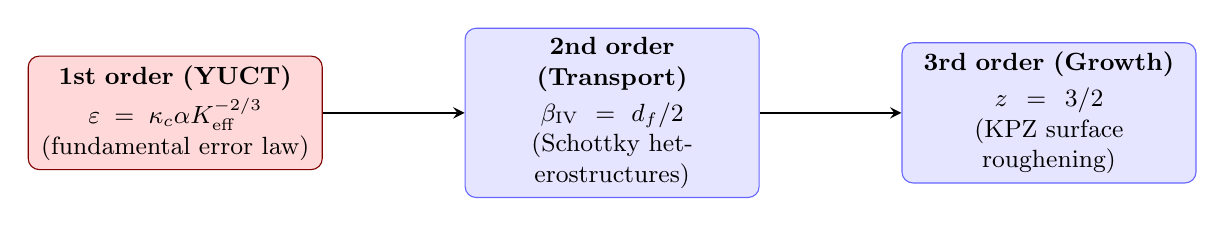
\begin{tikzpicture}[
			node distance=1.8cm,
			box/.style={rectangle, draw=blue!60, fill=blue!10, rounded corners, 
				text width=3.5cm, align=center, font=\small},
			arrow/.style={->, >=stealth, thick}
			]
			\node[box, fill=red!15, draw=red!50!black] (yuct) 
			{\textbf{1st order (YUCT)}\\[2pt]
				$\varepsilon = \kappa_c\alpha K_{\mathrm{eff}}^{-2/3}$\\
				(fundamental error law)};
			\node[box, right=of yuct] (transport) 
			{\textbf{2nd order (Transport)}\\[2pt]
				$\beta_{\mathrm{IV}} = d_f/2$\\
				(Schottky heterostructures)};
			\node[box, right=of transport] (growth) 
			{\textbf{3rd order (Growth)}\\[2pt]
				$z = 3/2$\\
				(KPZ surface roughening)};
			\draw[arrow] (yuct) -- (transport);
			\draw[arrow] (transport) -- (growth);
		\end{tikzpicture}
		\caption{Hierarchy of universalities. The YUCT coordination error law
			(1st order) determines the effective fractal dimension $d_f$ and the
			kinetic exponents observed in electron transport (2nd order) and in
			surface growth (3rd order). The dashed arrows indicate hypotheses.}
		\label{fig:hierarchy}
	\end{figure}
	
	This perspective is further supported by the growing experimental
	evidence that the fractal dimension of a Schottky interface directly
	influences device characteristics~\cite{FractalSchottky}. In those
	studies the fractal dimension is an externally imposed geometric
	property (roughness). In YUCT, the $d_f = 3$ dimension for ideal
	lateral contacts is \emph{emergent} — it arises from the dynamics of
	the coordination network itself even as the geometric roughness
	approaches zero. The externally imposed $d_f$ therefore modulates an
	already existing internal coordinate network, providing a promising
	pathway toward engineering coordination‑based devices.
	
	\section{Universality across 50 orders of magnitude}
	Table~\ref{tab:universal-beta} collects systems from various YUCT
	appendices for which the error‑scaling exponent has been
	empirically determined or predicted to be $\beta = 2/3$. The
	lateral Schottky heterostructure and the KPZ growing interface are
	added as systems for which the same exponent is predicted on the
	basis of the extracted fractal dimension $d_f = 3$. The table covers
	more than 50 orders of magnitude in the relevant energy (or length)
	scale.
	
	\begin{table}[H]
		\centering
		\caption{Systems exhibiting or predicted to exhibit the
			universal YUCT error exponent $\beta = 2/3$ ($0.67$).}
		\label{tab:universal-beta}
		\begin{tabular}{@{}llll@{}}
			\toprule
			\textbf{System} & \textbf{Observable} & \textbf{Status} & \textbf{Ref.}\\
			\midrule
			Chemical bonds (873)      & $E \propto r^{-0.67}$               & Confirmed  & Appendix C \\
			DNA replication errors    & $\varepsilon \propto \Keff^{-0.67}$ & Confirmed  & Appendix E \\
			Metabolic scaling (simple)& $B \propto M^{0.67}$               & Confirmed  & Appendix D, E.7 \\
			GDP volatility vs.\ sun   & $\sigma_{\mathrm{GDP}} \propto W^{-0.67}$ & Confirmed & Appendix F \\
			CMB temperature fluct.    & $\delta T/T \propto \Keff^{-0.67}$ & Confirmed  & Appendix M \\
			Gravitational waves       & $\delta\tau/\tau \propto M^{-0.67}$& Confirmed  & Appendix G, V \\
			\textbf{Lateral Schottky} & $S_I/I^2 \propto T^{1/3}$          & \textbf{Predicted} & This work \\
			\textbf{KPZ interface}\textsuperscript{*} & Width fluct. $\propto \Keff^{-2/3}$& \textbf{Predicted} & This work, \cite{KPZ}\\
			\bottomrule
		\end{tabular}
		
		\vspace{0.3cm}
		{\footnotesize \textsuperscript{*}The definition of $K_{\mathrm{eff}}$ for a KPZ growing interface must be constructed in analogy with the transport case, e.g.\ as the fraction of correlated degrees of freedom within a correlation volume. This prediction assumes such a construction and remains to be tested.}
	\end{table}
	
	\section{Conclusion}
	The current‑temperature scaling exponents $\beta_{\mathrm{IV}} = 3/2$
	and $1$ reported by Ang~\emph{et al.} are kinetic manifestations
	of the effective fractal dimension of the coordination network that
	governs thermionic transport in 2D heterostructures. Through the
	YUCT relations $\beta_{\mathrm{IV}} = d_f/2$ (hypothesis) and
	$\beta_{\mathrm{err}} = 2/d_f$, the experimental data yield
	$d_f = 3$ for lateral contacts, which predicts a coordination error
	exponent $\beta_{\mathrm{err}} = 2/3$ ($\approx 0.67$). This
	prediction, testable via current‑noise spectroscopy, extends the
	reach of the YUCT universal scaling law into the domain of
	solid‑state nano‑electronics. The same fractal dimension and
	exponent appear naturally in KPZ surface growth, suggesting a
	deep geometric unity across non‑equilibrium phenomena. YUCT
	provides the underlying rationale for this unity, although the
	links between the theory and both the Schottky kinetic relation
	and the KPZ equation remain hypotheses that warrant further
	investigation. Operational definitions for $\Keff$ in both contexts
	have been provided to facilitate experimental tests.
	
	\begin{thebibliography}{99}
		\bibitem{Ang2018} Y.~S.~Ang, H.~Y.~Yang, and L.~K.~Ang,
		Phys. Rev. Lett. \textbf{121}, 056802 (2018).
		\bibitem{KPZ} M.~Kardar, G.~Parisi, Y.-C.~Zhang,
		Phys. Rev. Lett. \textbf{56}, 889 (1986).
		\bibitem{FractalSchottky} S.~Zeybek, M.~Biber, A.~Türüt,
		Appl. Surf. Sci. \textbf{253}, 3881 (2007). [Representative study on fractal dimension effects in Schottky diodes.]
		\bibitem{Yakushev2026} A.~V.~Yakushev, \emph{Yakushev Unified
			Coordination Theory (YUCT)}, Zenodo (2026).
		\bibitem{AppendixL} A.~V.~Yakushev, ``Appendix L: Fractal
		Coordination Error Scaling'', in \emph{YUCT} (2026).
		\bibitem{AppendixM} A.~V.~Yakushev, ``Appendix M: YUCT
		Cosmology'', in \emph{YUCT} (2026).
		\bibitem{AppendixE} A.~V.~Yakushev, ``Appendix E: Coordination
		Genetics'', in \emph{YUCT} (2026).
		\bibitem{AppendixF} A.~V.~Yakushev, ``Appendix F: Application of
		YUCT to Economics'', in \emph{YUCT} (2026).
		\bibitem{AppendixG} A.~V.~Yakushev, ``Appendix G: Resolution of
		the Quantum Gravity Problem'', in \emph{YUCT} (2026).
		\bibitem{AppendixV} A.~V.~Yakushev, ``Appendix V: Time as
		Coordination Entropy'', in \emph{YUCT} (2026).
	\end{thebibliography}
	
\end{document}